





%
%
%  S  É  A  N  C  E     I
%
%



\section{Aide pour réaliser les activités}

\subsection{Aide pour la séance 1}\label{correction_scratch1}




Nous allons écrire le programme étape par étape.


\subsubsection{Modifier la scène où se passe l'action}\index{Scratch!Modifier la scène}\index{Modifier la scène (Scratch)}

La scène correspond à l'arrière-plan (blanc au départ) où se passe l'action. La scène est un objet qui peut être modifié. Pour cela, la première étape est de cliquer sur l'icône scène 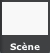
\includegraphics[width=1cm]{./images/scratch/Scene} en bas à droite.

\uneimageici{./images/scratch/ScratchSelectionScene}{.65\textwidth}

Une fois la scène sélectionnée (elle est alors entourée en couleur), suivre les 4 étapes suivantes :

\begin{enumerate}
\item Cliquer sur l'onglet \texttt{Arrière-plans}.
\item Cliquer sur le bouton \texttt{Importer}.
\item Choisir l'arrière-plan \texttt{xy-grid}.
\item Cliquer alors sur le bouton \texttt{OK}. 
\end{enumerate}


\uneimageici{./images/scratch/ScratchChangerScene1}{.8\textwidth}

Notre programme comporte maintenant deux scènes différentes : \texttt{arrière-plan1} et \texttt{xy-grid}. C'est cette dernière qui est sélectionnée (elle est entourée en couleur).

\uneimageici{./images/scratch/ScratchChangerScene2}{.4\textwidth}






\subsubsection{Enregistrer le programme}\index{Enregistrer!Scratch}\index{Scratch!Enregistrer}

Pour sauvegarder votre programme : cliquer sur l'icône 
\includegraphics[width=.4cm]{./images/scratch/Sauver} :

\uneimageici{./images/scratch/ScratchEnregistrerProgramme1}{.5\textwidth}

Il faut ensuite choisir l'emplacement \emph{Bureau} de l'ordinateur, puis donner un nom au fichier dans lequel votre programme sera sauvegardé :

\uneimageici{./images/scratch/ScratchEnregistrerProgramme2}{.7\textwidth}


Comme toujours en informatique, il ne faut pas oublier d'enregistrer régulièrement le travail. Pour cela, cliquer régulièrement sur l'icône 
\includegraphics[width=.4cm]{./images/scratch/Sauver} ou utiliser la combinaison de touche \texttt{Cmd + S} :

\uneimageici{./images/generales/clavierCmdS}{.4\textwidth}









\subsubsection{Ajouter un script associé au lutin}\label{ScriptLutin}\index{Scratch!Script associé à un objet}\index{Script associé à un objet (Scratch)}

Le lutin est un autre objet. C'est lui qui réalise l'action principale du programme. On va lui associer un programme (nommé \textbf{script}) qui contient une succession d'ordres (les \textbf{instructions}) qu'il devra réaliser.  

Pour construire ce premier script, suivre les différentes étapes indiquées sous l'image ci-dessous.

\uneimageici{./images/scratch/ScratchPremierProgramme1}{.8\textwidth}

\begin{enumerate}
\item Sélectionner le lutin 
\includegraphics[width=.7cm]{./images/scratch/Lutin} dans la zone des objets (colonne 3) : nous allons créer un script associé au lutin.
\item Choisir les blocs de contrôle en cliquant sur 
\includegraphics[width=2cm]{./images/scratch/BlocsControle} (colonne 1).
\item Tirer le bloc 
\includegraphics[width=2.5cm]{./images/scratch/BlocDrapeauVert} vers la zone de programmation (colonne 2).
\item Choisir les blocs de mouvement en cliquant sur 
\includegraphics[width=2cm]{./images/scratch/BlocsMouvement} (colonne 1).
\item Tirer le bloc 
\includegraphics[width=2.5cm]{./images/scratch/BlocAllerA} vers la zone de programmation et l'accrocher sous le bloc 
\includegraphics[width=2.5cm]{./images/scratch/BlocDrapeauVert}.
\item Tirer ensuite le bloc 
\includegraphics[width=4.5cm]{./images/scratch/BlocGlisser} vers la zone de programmation et l'accrocher sous le bloc 
\includegraphics[width=2.5cm]{./images/scratch/BlocAllerA}.
\item Régler les options du bloc en cliquant dans les zones de saisie et en écrivant la valeur de durée et les coordonnées $x$ et $y$ indiquées dans le programme ci-dessus.
\item Ajouter les trois autres blocs 
\includegraphics[width=4.5cm]{./images/scratch/BlocGlisser} et régler leurs options comme indiqué plus haut.
\item Choisir les blocs de sons en cliquant sur 
\includegraphics[width=2cm]{./images/scratch/BlocsSons} (colonne 1).
\item Tirer le bloc 
\includegraphics[width=4.5cm]{./images/scratch/BlocJouerTambour} vers la zone de programmation, l'accrocher aux blocs précédents et régler ses options comme indiqué plus haut.
\end{enumerate}

\vspace{12pt}

Après avoir terminé et vérifié le script, lancer le programme en appuyant sur le drapeau vert 
\includegraphics[width=.7cm]{./images/scratch/DrapeauVert} en haut à droite. Aviez-vous deviné correctement ce qu'il allait se passer ?

Pour arrêter l'exécution du programme avant sa fin, appuyer sur le panneau stop 
\includegraphics[width=.7cm]{./images/scratch/Stop} en haut à droite.

Pour que le programme s'exécute en plein écran, cliquer sur 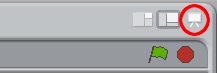
\includegraphics[width=3cm]{./images/scratch/ScratchPleinEcran}\index{Scratch! Passer en mode plein écran}\index{Passer en mode plein écran (Scratch)}

Pour quitter le mode plein écran, cliquer sur 
\includegraphics[width=1.5cm]{./images/scratch/ScratchQuitterPleinEcran}\index{Scratch! Quitter le mode plein écran}\index{Quitter le mode plein écran (Scratch)}








\subsubsection{Ajouter un script associé à la scène}\index{Scratch!Script associé à la scène}\index{Script associé à la scène (Scratch)}

Nous allons maintenant ajouter un deuxième script à notre programme : ce script va permettre de modifier la scène lorsque le drapeau vert est pressé. 

Pour cela, la première étape est de cliquer sur l'icône scène 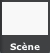
\includegraphics[width=1cm]{./images/scratch/Scene} en bas à droite.

\uneimageici{./images/scratch/ScratchPremierProgramme2}{.7\textwidth}

Une fois la scène sélectionnée (elle est alors entourée en couleur), créer le script suivant :

\uneimageici{./images/scratch/ScratchProgramme1Script2}{.4\textwidth}

Une fois le script écrit et vérifié, lancer le programme en appuyant sur le drapeau vert 
\includegraphics[width=.7cm]{./images/scratch/DrapeauVert} en haut à droite. 








%
%
%  S  É  A  N  C  E     II
%
%









\subsection{Aide pour la séance 2}\label{correction_scratch2}


Construire le script : puisqu'il est associé à l'objet lutin, vérifier qu'il est bien sélectionné avant de le construire (voir si nécessaire le paragraphe \vref{ScriptLutin} pour sélectionner le lutin avant de construire le programme). Pour construire le bloc 
\includegraphics[width=6cm]{./images/scratch/ScratchActivite23}, il faut procéder en deux temps :

\begin{enumerate}
\item Positionner les deux blocs d'instructions \texttt{pointer en direction...} et \texttt{nombre aléatoire entre...} dans la zone de programme ;

\uneimageici{./images/scratch/ScratchActivite21}{.6\textwidth}

\item Tirer le bloc \texttt{nombre aléatoire entre...} dans la zone de saisi du bloc \texttt{pointer en direction...}

\uneimageici{./images/scratch/ScratchActivite22}{.5\textwidth}

Il suffit ensuite de régler les valeurs et d'accrocher le bloc obtenu sous le bloc \texttt{abaisser le stylo}.
\end{enumerate}



Une fois que vous avez terminé et vérifié le script, lancer le programme en appuyant sur le drapeau vert 
\includegraphics[width=.7cm]{./images/scratch/DrapeauVert} en haut à droite. Aviez-vous deviné correctement ce qu'il allait se passer ?




\subsubsection{Ajouter l'effacement de l'écran}

À côté du script précédent, construire le script ci-dessous qui permet d'effacer l'écran lorsque la touche \texttt{Espace} est pressée.

\uneimageici{./images/scratch/ScratchScriptCarre2}{.25\textwidth}






\subsubsection{Un carré où on veut !}

En utilisant les instructions ci-dessous, modifier le script pour que le carré soit dessiné à l'endroit où se trouve le pointeur de la souris.

\uneimageici{./images/scratch/ScratchScriptCarre3}{.25\textwidth}


\subsubsection{Dessiner une enveloppe}

Créer un nouveau script, toujours pour l'objet lutin, qui permette de dessiner une enveloppe identique à celle ci-dessous. Le but est de réaliser cette enveloppe sans jamais lever le crayon ni repasser deux fois sur le même trait.

\uneimageici{./images/scratch/enveloppe}{.25\textwidth}




\subsubsection{Modifier la taille et la couleur du stylo}

En utilisant les instructions suivantes, modifier la couleur des traits et la taille du crayon.

\uneimageici{./images/scratch/ScratchEnveloppeTailleCrayon}{.35\textwidth}










%
%
%  S  É  A  N  C  E     III
%
%









\subsection{Aide pour la séance 3}\label{correction_scratch3}



\subsubsection{Ajouter un nouvel objet : l'avion}\index{Scratch!Ajouter et éditer un objet}\index{Ajouter et éditer un objet (Scratch)}

\begin{enumerate}
\item Sélectionner l'objet lutin.
\item Choisir l'onglet \texttt{Costume}, puis appuyer sur le bouton \texttt{Importer}.
\item Dans le dossier \texttt{Transportation}, choisir l'avion 
\includegraphics[width=1cm]{./images/scratch/Avion} puis valider en cliquant sur le bouton \texttt{OK} :
\uneimageici{./images/scratch/ScratchCostumeAvion1}{.8\textwidth}
\item Supprimer alors l'objet lutin en cliquant sur le bouton 
\includegraphics[width=.7cm]{./images/scratch/Supprimer} :
\uneimageici{./images/scratch/ScratchSupprimerLutin}{.5\textwidth}
\item Appuyer sur le bouton \texttt{Édition} à côté de l'avion, puis réduire la taille de l'avion en appuyant 8 fois sur le bouton 
\includegraphics[width=1cm]{./images/scratch/Reduire} :
\uneimageici{./images/scratch/ScratchReduireTailleAvion}{.8\textwidth}
\end{enumerate}
On a maintenant un petit avion (objet remplaçant le lutin), sur un fond blanc (objet scène).

Vérifier que l'objet avion est bien sélectionné et cliquer sur l'onglet \texttt{Script} :

\uneimageici{./images/scratch/ScratchSelectionAvion}{.6\textwidth}






\subsubsection{Gérer les mouvements de l'avion dans la scène}  

On va maintenant ajouter un script pour notre avion. Puisque durant la partie, l'avion doit toujours avancer, nous allons utiliser une \textbf{boucle infinie}.\index{Scratch!Boucle infinie}\index{Boucle infinie (Scratch)}

\vspace{12pt}

\cadre{La \textbf{boucle} est une structure importante en programmation : elle permet de répéter un bloc d'instructions plusieurs fois, tant qu'une condition est vérifiée ou même indéfiniment. Dans notre programme, nous utilisons une boucle infinie.\uneimageici{./images/scratch/ScratchBoucle}{.6\textwidth}}  

\vspace{12pt}



\begin{enumerate}
\item Construire le script suivant associé à l'objet avion (il faut donc que l'objet avion soit sélectionné) :
\uneimageici{./images/scratch/ScratchActivite31}{.3\textwidth}
\item Ajouter les deux scripts suivants, également associés à l'objet avion :
\uneimageici{./images/scratch/ScratchActivite32}{.7\textwidth}
\item Pour tester votre programme, démarrer en appuyant sur le drapeau vert 
\includegraphics[width=.7cm]{./images/scratch/DrapeauVert} en haut à droite. Appuyer sur le panneau stop 
\includegraphics[width=.7cm]{./images/scratch/Stop} en haut à droite pour mettre fin au programme.
\end{enumerate}

Pour que le programme s'exécute en plein écran, cliquer sur 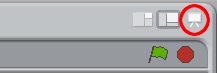
\includegraphics[width=3cm]{./images/scratch/ScratchPleinEcran}

Pour quitter le mode plein écran, cliquer sur 
\includegraphics[width=1.5cm]{./images/scratch/ScratchQuitterPleinEcran}


\subsubsection{Un nouvel objet : l'obstacle}\index{Scratch!Créer un objet}\index{Créer un objet (Scratch)}       

On va maintenant ajouter un obstacle que l'avion devra éviter.

\begin{enumerate}
\item Ajouter un nouvel objet en appuyant sur l'étoile 
\includegraphics[width=.7cm]{./images/scratch/EtoilePinceau} :
\uneimageici{./images/scratch/ScratchActivite33}{.8\textwidth}
\item Créer un petit rectangle de la couleur de votre choix.
\uneimageici{./images/scratch/ScratchCreerRectangle}{.6\textwidth}
Terminer en appuyant sur le bouton \texttt{OK}
\item Nous avons maintenant un nouvel objet nommé \texttt{Objet2} :
\uneimageici{./images/scratch/ScratchActivite34}{.4\textwidth}
\item Sélectionner à nouveau l'objet 1 car c'est à lui que nous allons associer un nouveau script.
\end{enumerate}


\subsubsection{Gérer la collision entre l'avion et l'obstacle}\index{Scratch!Collision entre objets}\index{Collision entre objets (Scratch)} 

On va maintenant traiter le cas où l'avion entre en collision avec l'objet 2. La partie sera alors perdue. Nous allons utiliser ici une \textbf{structure conditionnelle} : un bloc d'instructions sera exécuté \emph{si} la condition \emph{objet 1 percute objet 2} est vérifiée.\index{Scratch!Structure conditionnelle \emph{si}}\index{Structure conditionnelle \emph{si} (Scratch)} 

\vspace{12pt}

\cadre{La \textbf{structure conditionnelle <<\,si\,>>} est une structure importante en programmation : elle permet d'exécuter un bloc d'instructions \textbf{si} une condition est vérifiée.\uneimageici{./images/scratch/ScratchSi}{.55\textwidth}}  

\vspace{12pt}





\begin{enumerate}
\item Modifier le script pour qu'il corresponde à celui ci-dessous. Le bloc 
\includegraphics[width=2cm]{./images/scratch/BlocCapteur} se trouve dans les blocs \texttt{Capteur} (colonne 1).
\uneimageici{./images/scratch/ScratchActivite35}{.4\textwidth}
\item On ne veut pas le son par défaut \texttt{miaou} mais plutôt un son qui annonce que la partie est perdue. Pour cela, il faut enregistrer un nouveau son. Cliquer sur la flèche à droite du nom du son...
\uneimageici{./images/scratch/ScratchActiviteSonChanger}{.2\textwidth}

...puis choisir \texttt{enregistrer...}

\uneimageici{./images/scratch/ScratchActivite36}{.4\textwidth}
\item Démarrer l'enregistrement à l'aide du bouton 
\includegraphics[width=.7cm]{./images/scratch/SonEnregistre}, dire \emph{<<\,Perdu !\,>>}, puis l'arrêter à l'aide du bouton 
\includegraphics[width=.7cm]{./images/scratch/SonStop}. Faire plusieurs essais jusqu'à être satisfait du son enregistré.
\uneimageici{./images/scratch/ScratchActivite37}{.8\textwidth}
\item Un nouveau son nommé \texttt{enregistrement1} est maintenant disponible. On peut alors supprimer le son \texttt{miaou} en cliquant sur le bouton 
\includegraphics[width=.7cm]{./images/scratch/Supprimer} :
\uneimageici{./images/scratch/ScratchActivite38}{.4\textwidth}
\item On ajoute encore un quatrième et dernier script associé à l'\texttt{Objet 1}. Ce script permet de repositionner l'avion lorsque la touche \texttt{espace} est pressée :
\uneimageici{./images/scratch/ScratchActivite39}{.3\textwidth}
\end{enumerate}













